% Crouch et al. (2022) scatter (../jeffScatter.png, 1360x632 px): removes the
% (a)/(b) panel labels and marks the right panel as a zoom of the left one
% (w/delta* in [0,50], d/delta* in [0,5]).
% Build: pdflatex jeffScatterZoom.tex && cp jeffScatterZoom.pdf ../jeffScatterZoom.pdf
\documentclass{standalone}
\usepackage{tikz}
\begin{document}
\begin{tikzpicture}[x=1bp, y=-1bp]
	% 1 px = 1 bp, origin at the top-left corner of the image
	\node[anchor=north west, inner sep=0pt] at (0,0) {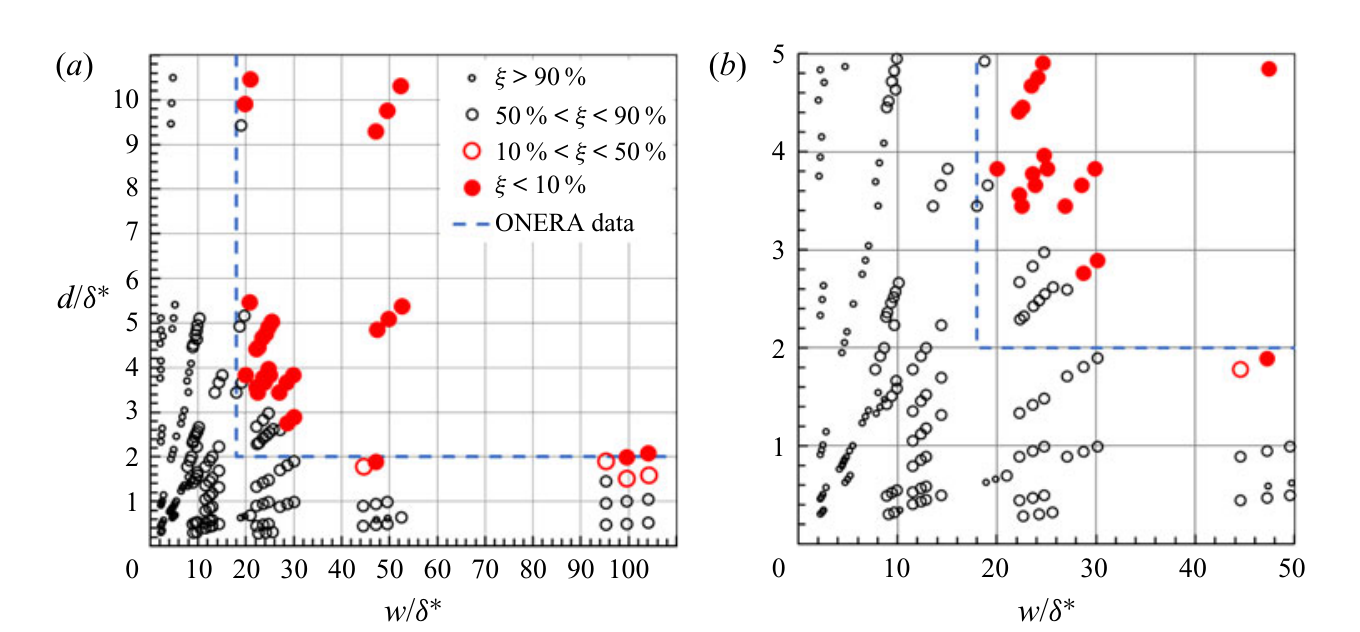
\includegraphics[width=1360bp]{../jeffScatter.png}};
	\fill[white] (48,38) rectangle (100,90);    % (a)
	\fill[white] (702,38) rectangle (752,90);   % (b)
	% Left axes: w = 0 at x = 149.5, 4.79 px per unit; d = 0 at y = 545.5, 44.6 px per unit
	\coordinate (zTL) at (149.5,322.5);  \coordinate (zTR) at (389,322.5);
	\coordinate (zBL) at (149.5,545.5);  \coordinate (zBR) at (389,545.5);
	% Right axes frame
	\coordinate (rTL) at (797.5,53.5);   \coordinate (rBL) at (797.5,543.5);
	% tab:orange: no data or reference line in the plot uses it
	\definecolor{zoomcolor}{RGB}{255,127,14}
	\begin{scope}[zoomcolor, line width=4bp]
		\draw (zBL) rectangle (zTR);
		\draw[line width=2.5bp] (zTR) -- (rTL);
		\draw[line width=2.5bp] (zBR) -- (rBL);  % runs along the left x-axis
	\end{scope}
\end{tikzpicture}
\end{document}
